\documentclass[../Proposal.tex]{subfiles}
 
\begin{document}
\section{Single Linkage Clustering}
Merupakan salah satu metode dari \textit{hierarchical clustering}\cite{introduction-information-retrieval} yang bekerja dengan cara \textit{bottom-up}. Setiap elemen yang ada dianggap sebagai \textit{cluster} yang berdiri sendiri. \textit{Clustering} akan dilakukan dengan menggabungkan jarak terdekat elemen 2 \text{cluster} dari seluruh yang ada, hingga menjadi 1 \textit{cluster}. Gambar \ref{fig:dendogram} menunjukan contoh \textit{clustering} yang dilakukan pada 30 buah dokumen. 

\begin{figure}[H]
	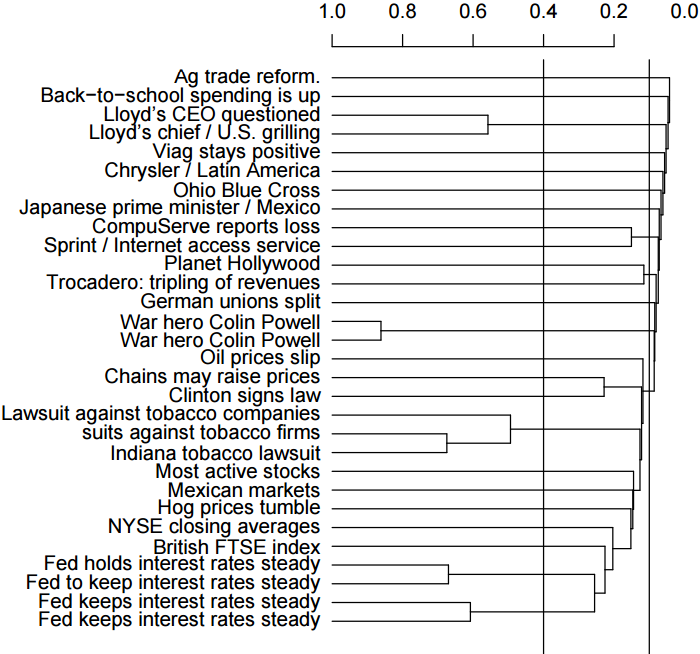
\includegraphics[width=.9\linewidth]{../images/dendogram}
	\caption{Contoh \textit{Dendogram} dari \textit{Single Linkage Clustering}\cite{introduction-information-retrieval}}
	\label{fig:dendogram}
\end{figure}

\noindent Untuk tugas akhir ini penggabungan \textit{cluster} yang ada menggunakan jarak yang dinotasikan\cite{dist} oleh Persamaan \ref{eq:dmin}. 

\begin{center}
	\begin{equation}
		D(X,Y)=min\ d(x,y) ;\ x \in X, y \in Y
		\label{eq:dmin}
	\end{equation}
\end{center}
Atau dapat digambarkan seperti pada Gambar \ref{fig:dist}
\begin{center}
	\begin{figure}[H]
		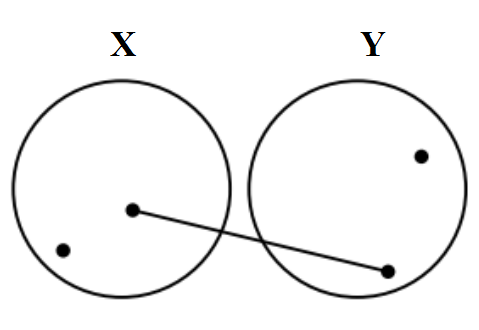
\includegraphics[width=.4\linewidth]{../images/repSingle}
		\caption{Representasi \textit{Single Linkage Clustering}}
		\label{fig:dist}
	\end{figure}
\end{center}

\noindent Selain itu pada tugas akhir ini yang menjadi kondisi terminasi adalah $D(X,Y)$. Apabila jarak terpendek pada \textit{cluster} $\geq \gamma$, maka proses \textit{cluster} terhenti. Gambar \ref{fig:scl} menunjukan contoh proses \textit{clustering} dengan \textit{Single Linkage Clustering}.

\begin{figure}[H]
	\centering
	
	
	\begin{subfigure}{.5\textwidth}
		\centering
		\includegraphics[width=.7\linewidth]{../images/c1}
		\caption{Step-0}
	\end{subfigure}%
	\begin{subfigure}{.5\textwidth}
		\centering
		\includegraphics[width=.7\linewidth]{../images/c2}
		\caption{Step-1}
	\end{subfigure}
	
	\centering
	\begin{subfigure}{.5\textwidth}
		\centering
		\includegraphics[width=.7\linewidth]{../images/c3}
		\caption{Step-2}
	\end{subfigure}%
	\begin{subfigure}{.5\textwidth}
		\centering
		\includegraphics[width=.7\linewidth]{../images/c4}
		\caption{Step-3}
	\end{subfigure}

	\centering
	\begin{subfigure}{.5\textwidth}
		\centering
		\includegraphics[width=.7\linewidth]{../images/c5}
		\caption{Step-4}
	\end{subfigure}
\caption{Contoh Proses \textit{Clustering}}
\label{fig:scl}

\end{figure}

\noindent Gambar \ref{fig:endcl} merupakan hasil akhir dari proses \textit{clustering} di atas.

	\begin{figure}[H]
		\includegraphics[width=.45\linewidth]{../images/cResult}
		\caption{\textit{Cluster} Akhir}
		\label{fig:endcl}
	\end{figure}
\end{document}